% A '%' character causes TeX to ignore all remaining text on the line,
% and is used for comments like this one.

\documentclass{article}      % Specifies the document class
\usepackage{amsmath, nccmath}
\usepackage{enumitem}
\usepackage{graphicx}
\usepackage[utf8]{inputenc}
\usepackage{listings}
\usepackage{xcolor}
\graphicspath{ {./} }
\definecolor{codegreen}{rgb}{0,0.6,0}
\definecolor{codegray}{rgb}{0.5,0.5,0.5}
\definecolor{codepurple}{rgb}{0.58,0,0.82}
\definecolor{backcolour}{rgb}{0.95,0.95,0.92}
\usepackage{float}
\lstdefinestyle{mystyle}{
    backgroundcolor=\color{backcolour},   
    commentstyle=\color{codegreen},
    keywordstyle=\color{magenta},
    numberstyle=\tiny\color{codegray},
    stringstyle=\color{codepurple},
    basicstyle=\ttfamily\footnotesize,
    breakatwhitespace=false,         
    breaklines=true,                 
    captionpos=b,                    
    keepspaces=true,                 
    numbers=left,                    
    numbersep=5pt,                  
    showspaces=false,                
    showstringspaces=false,
    showtabs=false,                  
    tabsize=2
}

\lstset{style=mystyle}

\title{CEE 498 Applied Machine Learning - HW5}  % Declares the document's title.
\author{Rini Jasmine Gladstone (rjg7) and Maksymillian Podraza(podraza3)}      % Declares the author's name.
\date{April 17, 2020}      % Deleting this command produces today's date.

\newcommand{\ip}[2]{(#1, #2)}
                             % Defines \ip{arg1}{arg2} to mean
                             % (arg1, arg2).

%\newcommand{\ip}[2]{\langle #1 | #2\rangle}
                             % This is an alternative definition of
                             % \ip that is commented out.

\begin{document}             % End of preamble and beginning of text.

\maketitle                   % Produces the title.


\section{Problem 1}      % Produces section heading.  Lower-level
                             % sections are begun with similar 
                             % \subsection and \subsubsection commands.

\subsection{Part a}

We used the following image for our analysis.

\begin{figure}[H]
\centering
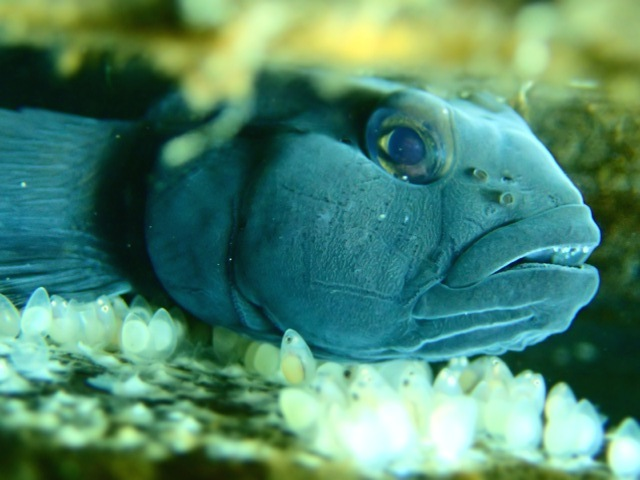
\includegraphics[width=0.7\textwidth]{RobertMixed03.jpg}
\end{figure}

We normalized the image so that the darkest pixel takes the value (0,0,0) and the lightest pixel takes the value (1,1,1).

\begin{lstlisting}
image_paths = ["RobertMixed03.jpg", "smallstrelitzia.jpg", "smallsunset.jpg"]

def load_images():
    image_array = []
    try:
        for image_path in image_paths:
            img = Image.open(image_path)
            image_array.append(img)
    except IOError: 
        pass
    return image_array

images = load_images()

working_image = images[0]

def image_matrix_create(image):
    image_matrix = []
    img_w, img_h = image.size
    image_data = list(image.getdata())
    for y in range(img_h):
        image_matrix.append(image_data[y*img_w:(y+1)*img_w])
    image_df = pd.DataFrame(image_matrix)
    return image_df

def rgb_extract(image):
    rgb = []
    for i in range(3):
        rgb.append(image.apply(lambda x: [y[i] for y in x]))
    return rgb

def rgb_normalize(image):
    normalized = []
    for i in range(3):
        x = image[i].values 
        min_max_scaler = preprocessing.MinMaxScaler()
        x_scaled = min_max_scaler.fit_transform(x)
        df = pd.DataFrame(x_scaled)
        normalized.append(df)
    return normalized

r = image_matrix_create(working_image)
rgb_matrix_list = rgb_extract(r)
rgb_normalized_list = rgb_normalize(rgb_matrix_list)
\end{lstlisting}

Then, we wrote the function for EM. We used K means to initialize the mean vector. 
\begin{lstlisting}
def EM_function(X,cov,k,niter):    
        weights = np.ones((k)) / k
        kmeans = KMeans(n_clusters=k)
        # fit kmeans object to data
        kmeans.fit(X)
        means = kmeans.cluster_centers_
        eps=1e-8
        likelihood = []
        log_likelihoods = []
        for step in range(niter):
            likelihood = []
            # Expectation step
            for j in range(k):
                likelihood.append(multivariate_normal.pdf(x=X, mean=means[j], cov=cov[j]))
            likelihood = np.array(likelihood)
            assert likelihood.shape == (k, len(X))
            b = []
            # Maximization step 
            for j in range(k):
                # use the current values for the parameters to evaluate the posterior
                # probabilities of the data have been generated by each gaussian
                b.append((likelihood[j] * weights[j]) / (np.sum([likelihood[i] * weights[i] for i in range(k)], axis=0)+eps))
                # update mean and variance
                means[j] = np.sum(b[j].reshape(len(X),1) * X, axis=0) / (np.sum(b[j]+eps))
                # update the weights
                weights[j] = np.mean(b[j])
                assert cov.shape == (k, X.shape[1], X.shape[1])
                assert means.shape == (k, X.shape[1])
            log_likelihoods.append(np.log(np.sum([k*multivariate_normal(means[i],cov[j]).pdf(X) for k,i,j in zip(weights,range(len(means)),range(len(cov)))])))
            if (step+1)%100==0 and (step+1)>=100:
                print(step+1)
        return means,weights,b,log_likelihoods,likelihood
\end{lstlisting}

We set the covariance matrix (cov) to be identity matrix and ran the following code setting k = 10, 20 and 50.

\begin{lstlisting}
rvalues=rgb_normalized_list[0].values.flatten()
gvalues=rgb_normalized_list[1].values.flatten()
bvalues=rgb_normalized_list[2].values.flatten()
list_of_tuples = list(zip(rvalues, gvalues, bvalues))  
data=pd.DataFrame(list_of_tuples, columns = ['R', 'G', 'B'])
#Number of clusters
k=50
#Initializing the covariance matrix
cov = []
for i in range(k):
    cov.append(np.eye(data.shape[1]))
cov = np.array(cov)
means,weights,b,log_likelihoods,likelihood=EM_function(data,cov,k,200)
#Plotting the log-likelihood
plt.plot(log_likelihoods)
likelihood = np.array(likelihood)
#Finding the closest cluster for each pixel
predictions = np.argmax(likelihood, axis=0)
data['cluster']=predictions
data['mean_R']=np.zeros(data.shape[0])
data['mean_G']=np.zeros(data.shape[0])
data['mean_B']=np.zeros(data.shape[0])
for i in range(data.shape[0]):
    data.at[i,'mean_R']=means[data.at[i,'cluster']][0]
    data.at[i,'mean_G']=means[data.at[i,'cluster']][1]
    data.at[i,'mean_B']=means[data.at[i,'cluster']][2]
for i in range(k):
    data['weight_c'+str(i)]=b[i]
\end{lstlisting}

We ran the code for 200 iterations. 

The following are the images obtained by replacing each pixel with the mean of its cluster center.     

   
\begin{figure}[H]
\centering
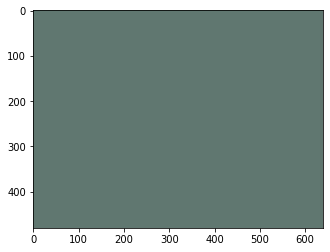
\includegraphics[width=0.7\textwidth]{fish_parta_means_10}
\caption{10 Clusters}
\end{figure}

   
\begin{figure}[H]
\centering
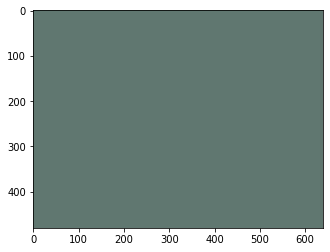
\includegraphics[width=0.7\textwidth]{fish_parta_means_20}
\caption{20 Clusters}
\end{figure}

    
\begin{figure}[H]
\centering
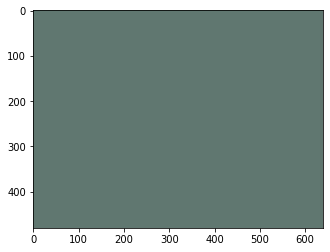
\includegraphics[width=0.7\textwidth]{fish_parta_means_50}
\caption{50 Clusters}
\end{figure}



The code for generating the above images is as shown below.

\begin{lstlisting}
def rescale_matrix(matrix, mode="int"):
    new_matrix = matrix
    for col in range(working_w):
        new_matrix.loc[:, col] *= 255
    
    if mode == "int":
        new_matrix.astype(int)
    return new_matrix
        

def print_matrix_image(original_image, image):
    im2 = Image.new(original_image.mode, original_image.size)
    img = image.values.flatten()
    im2.putdata(img)
    plt.imshow(im2)

def matricize_list(image, img_w=working_w, img_h=working_h):
    image_matrix = []
    for y in range(img_h):
        image_matrix.append(image[y*img_w:(y+1)*img_w])
    image_df = pd.DataFrame(image_matrix)
    return image_df
    return image_df


matrix_mean_R = matricize_list(list(data["mean_R"]))
matrix_mean_G = matricize_list(list(data["mean_G"]))
matrix_mean_B = matricize_list(list(data["mean_B"]))

matrix_mean_rescaled_R = rescale_matrix(matrix_mean_R)
matrix_mean_rescaled_G = rescale_matrix(matrix_mean_G)
matrix_mean_rescaled_B = rescale_matrix(matrix_mean_B)

matrix_mean_R = matrix_mean_R.astype(int)
matrix_mean_G = matrix_mean_G.astype(int)
matrix_mean_B = matrix_mean_B.astype(int)
matrix_mean_RGB = pd.DataFrame(np.rec.fromarrays((matrix_mean_R.values, matrix_mean_G.values, matrix_mean_B.values)).tolist(),
                      columns=matrix_mean_R.columns,
                      index=matrix_mean_R.index)

print_matrix_image(working_image, matrix_mean_RGB)
\end{lstlisting}

We observe from the figures that all the cluster centers have same mean, i.e. they drift together and hence the mean image is just a single color. Its the same for k=10,20 and 50

\subsection{Part b}

We constructed the figures showing the weights linking each pixel to each cluster center. Following is the code which executes this.

\begin{lstlisting}
fig = plt.figure(figsize=(12, 12))
gs = gridspec.GridSpec(5, 2)
gs.update(wspace=0.25, hspace=0.25)

for i in range(10):
    ax = plt.subplot(gs[i])
    a = data["weight_c"+str(i)].values.reshape(working_h,working_w)
    plt.axis('off')
    plt.title("Cluster "+ str(i+1))
    ax.set_aspect('equal')
    plt.imshow(a)
\end{lstlisting}

The images generated are as shown below.

\begin{figure}[H]
\centering
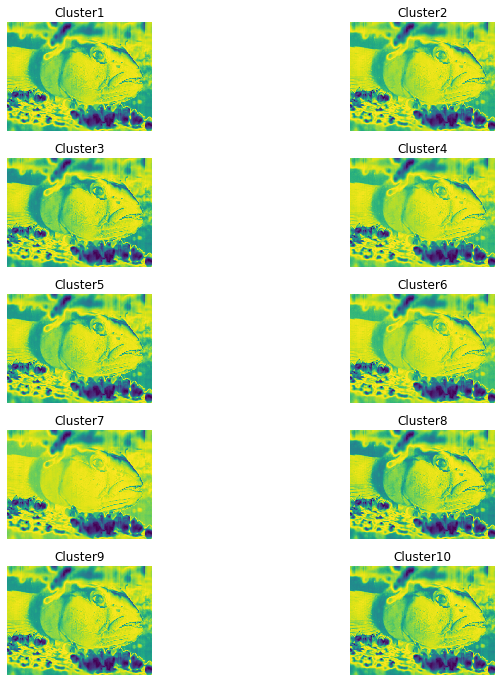
\includegraphics[width=0.7\textwidth]{fish_wts_partb}
\caption{Cluster 1}
\end{figure}

We can observe that all the weight maps look similar, which is the expected behavior as at this scale, all the pixels are essentially one cluster and hence the weights are the same.

\subsection{Part c}

We changed the covariance to \(0.1 I\) as well as  \(0.0025 I\) and ran the code. 

\begin{lstlisting}
rvalues=rgb_normalized_list[0].values.flatten()
gvalues=rgb_normalized_list[1].values.flatten()
bvalues=rgb_normalized_list[2].values.flatten()
list_of_tuples = list(zip(rvalues, gvalues, bvalues))  
data=pd.DataFrame(list_of_tuples, columns = ['R', 'G', 'B'])
#Number of clusters
k=50
#Initializing the covariance matrix
cov = []
for i in range(k):
    cov.append(0.1*np.eye(data.shape[1]))
cov = np.array(cov)
means,weights,b,log_likelihoods,likelihood=EM_function(data,cov,k,200)
#Plotting the log-likelihood
plt.plot(log_likelihoods)
likelihood = np.array(likelihood)
#Finding the closest cluster for each pixel
predictions = np.argmax(likelihood, axis=0)
data['cluster']=predictions
data['mean_R']=np.zeros(data.shape[0])
data['mean_G']=np.zeros(data.shape[0])
data['mean_B']=np.zeros(data.shape[0])
for i in range(data.shape[0]):
    data.at[i,'mean_R']=means[data.at[i,'cluster']][0]
    data.at[i,'mean_G']=means[data.at[i,'cluster']][1]
    data.at[i,'mean_B']=means[data.at[i,'cluster']][2]
for i in range(k):
    data['weight_c'+str(i)]=b[i]
\end{lstlisting}

We ran the code for 200 iterations. 

The following are the images obtained by replacing each pixel with the mean of its cluster center. 

\begin{figure}[H]
\centering
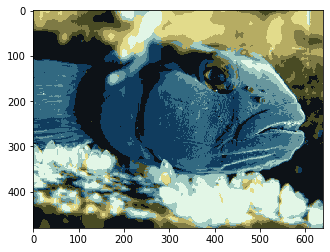
\includegraphics[width=0.7\textwidth]{fish_partc_means_10_400}
\caption{10 Clusters (0.0025 I)}
\end{figure}

\begin{figure}[H]
\centering
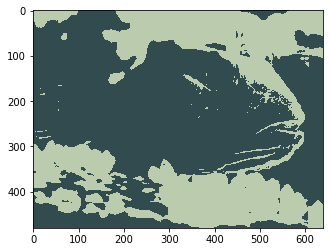
\includegraphics[width=0.7\textwidth]{fish_partc_means_10}
\caption{10 Clusters (0.1 I)}
\end{figure}

   
\begin{figure}[H]
\centering
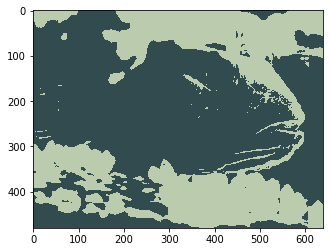
\includegraphics[width=0.7\textwidth]{fish_partc_means_20}
\caption{20 Clusters (0.1 I)}
\end{figure}

    
\begin{figure}[H]
\centering
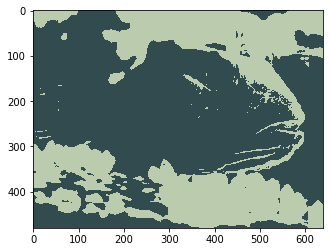
\includegraphics[width=0.7\textwidth]{fish_partc_means_50}
\caption{50 Clusters (0.1 I)}
\end{figure}


Following are the new set of weight maps.

\begin{figure}[H]
\centering
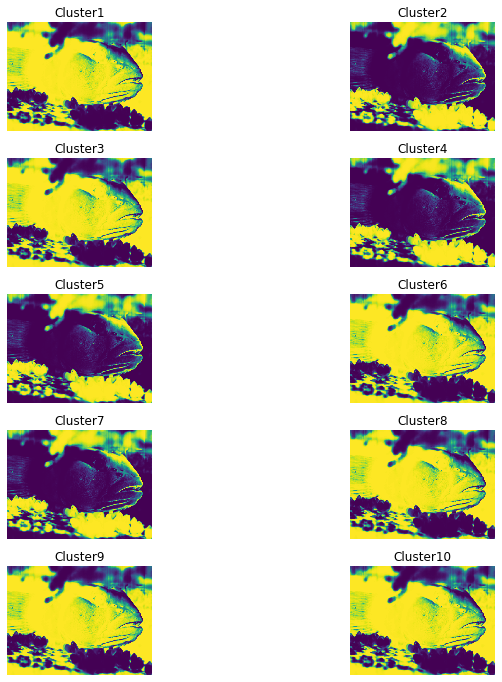
\includegraphics[width=0.7\textwidth]{fish_wts_partc_10}
\caption{Covariance = 0.1 I}
\end{figure}

\begin{figure}[H]
\centering
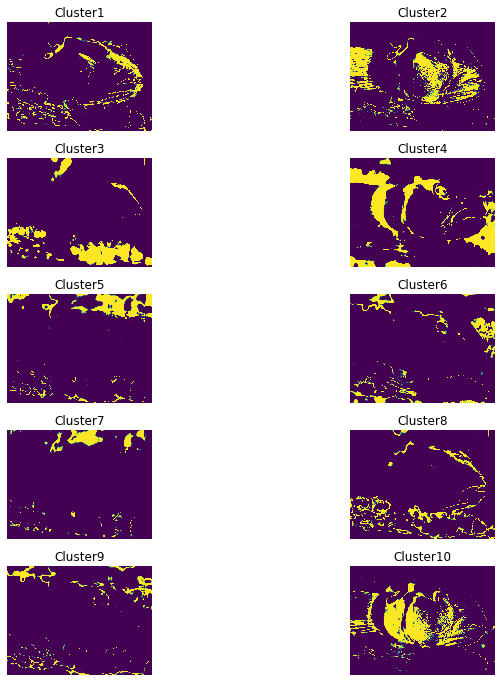
\includegraphics[width=0.7\textwidth]{fish_wts_partc_400}
\caption{Covariance = 0.0025 I}
\end{figure}

We can observe that for covariance = 0.1I, the weights are not so different. But as we change the covariance to 0.0025I, we observe variation in weights image across the clusters, which means that the cluster centers do not drift together for covariance = 0.0025I. This also resulted in a better recovery of image by replacing the pixels with the mean value (Figure 5).

\subsection{Part d}

We estimated the covariance of pixel values by assuming that pixels are normally distributed and clustered them using EM. The code for this is as given below.

\begin{lstlisting}
rvalues=rgb_normalized_list[0].values.flatten()
gvalues=rgb_normalized_list[1].values.flatten()
bvalues=rgb_normalized_list[2].values.flatten()
list_of_tuples = list(zip(rvalues, gvalues, bvalues))  
data=pd.DataFrame(list_of_tuples, columns = ['R', 'G', 'B'])
#Number of clusters
k=50
#Initializing the covariance matrix
cov = []
for i in range(k):
    cov.append(np.array(data.cov()))
cov = np.array(cov)
means,weights,b,log_likelihoods,likelihood=EM_function(data,cov,k,200)
#Plotting the log-likelihood
plt.plot(log_likelihoods)
likelihood = np.array(likelihood)
#Finding the closest cluster for each pixel
predictions = np.argmax(likelihood, axis=0)
data['cluster']=predictions
data['mean_R']=np.zeros(data.shape[0])
data['mean_G']=np.zeros(data.shape[0])
data['mean_B']=np.zeros(data.shape[0])
for i in range(data.shape[0]):
    data.at[i,'mean_R']=means[data.at[i,'cluster']][0]
    data.at[i,'mean_G']=means[data.at[i,'cluster']][1]
    data.at[i,'mean_B']=means[data.at[i,'cluster']][2]
for i in range(k):
    data['weight_c'+str(i)]=b[i]
\end{lstlisting}

 We ran the code for 200 iterations. 


The following are the images obtained by replacing each pixel with the mean of its cluster center. 

\begin{figure}[H]
\centering
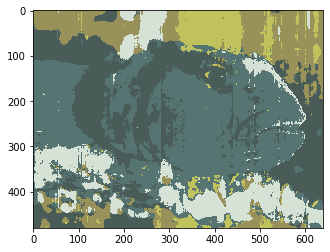
\includegraphics[width=0.7\textwidth]{fish_partd_means_10}
\caption{10 Clusters}
\end{figure}

   
\begin{figure}[H]
\centering
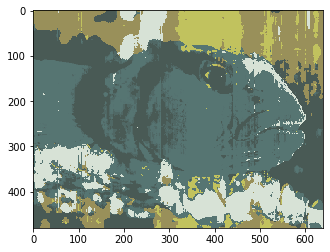
\includegraphics[width=0.7\textwidth]{fish_partd_means_20}
\caption{20 Clusters}
\end{figure}

    
\begin{figure}[H]
\centering
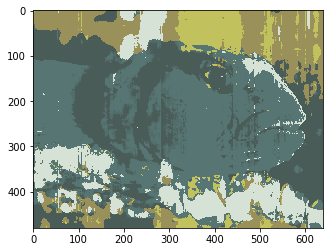
\includegraphics[width=0.7\textwidth]{fish_partd_means_50}
\caption{50 Clusters}
\end{figure}

Following are the new set of weight maps.

\begin{figure}[H]
\centering
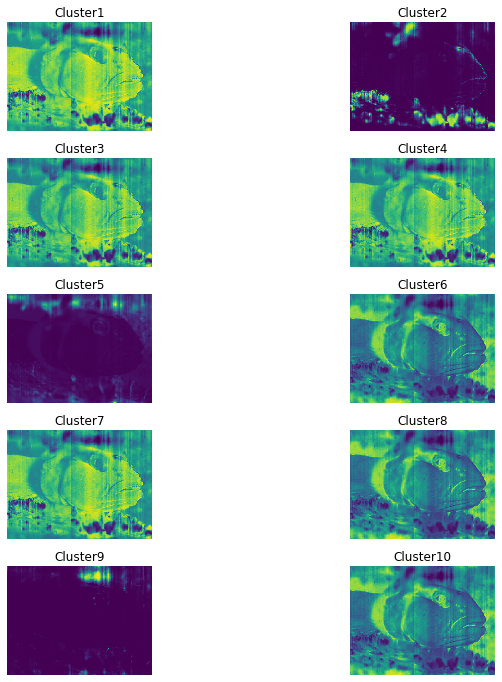
\includegraphics[width=0.7\textwidth]{fish_wts_partd}
\caption{}
\end{figure}

We observe that he centers do not drift, and the maps are different from each other. The mean image aloso has many colors and could recover the original image to an extent. This is very different from part a and b, where the centers drift together and the mean image is a single color.

\end{document}